\section{Esercizio 6 -- Sistema di lettura-elaborazione-scrittura}
\subsection{Esercizio 6.1}

L'obiettivo è realizzare un sistema sincrono che legge i dati da una memoria ROM, li trasforma con un'unità combinatoria M, e poi li memorizza in una memoria MEM. Il tutto è gestito da una unità di controllo [Figura \ref{fig:rom_m_mem}] che sincronizza le operazioni attraverso un contatore [Figura \ref{fig:6_1_ROM_M_MEM}].

\begin{figure}[h]
    \centering
    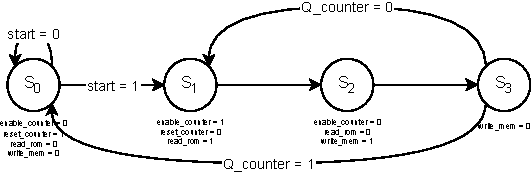
\includegraphics[width=0.6\textwidth]{img/rom_m_mem.pdf}
    \caption{Automa del sistema di lettura-elaborazione-scrittura}
    \label{fig:rom_m_mem}
\end{figure}

\begin{figure}[h]
    \centering
    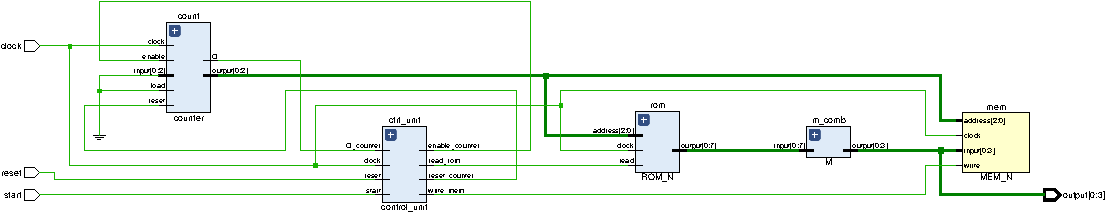
\includegraphics[width=\textwidth]{img/6_1_ROM_M_MEM.pdf}
    \caption{Schema a blocchi del sistema di lettura-elaborazione-scrittura}
    \label{fig:6_1_ROM_M_MEM}
\end{figure}

\subsubsection{Implementazione}

\begin{code}
    \inputminted{vhdl}{vhdl/rom_m_mem.vhd}
    \caption{Implementazione del sistema di lettura-elaborazione-scrittura}
    \label{cod:rom_m_mem}
\end{code}

\begin{code}
    \inputminted{vhdl}{vhdl/rom_m_mem_control_unit.vhd}
    \caption{Implementazione dell'unità di controllo}
    \label{cod:rom_m_mem_control_unit}
\end{code}

\begin{code}
    \inputminted{vhdl}{vhdl/rom_m_mem_M.vhd}
    \caption{Implementazione della macchina M}
    \label{cod:rom_m_mem_M}
\end{code}

Il sistema complessivo è implementato con un’architettura \texttt{structural} [Codice sorgente \ref{cod:rom_m_mem}], cioè connettendo più moduli (componenti) che lavorano insieme.
\paragraph{Funzionamento generale.}
Il sistema è progettato per avere il seguente funzionamento:

\begin{enumerate}
    \item Il sistema si avvia con un segnale di \texttt{start}.
    \item Un contatore scandisce progressivamente gli indirizzi della memoria ROM.
    \item Ad ogni indirizzo, il dato letto viene elaborato dall’unità M per ridurlo da 8 bit a 4 bit.
    \item Il risultato viene scritto nella memoria MEM, in corrispondenza dello stesso indirizzo.
    \item Il processo continua fino a quando tutte le N locazioni della ROM sono state lette e memorizzate in MEM.
\end{enumerate}

\paragraph{Struttura del codice.}
Il sistema, essendo implementato in maniera strutturale, presenta i seguenti moduli:

\begin{itemize}
    \item Unità di Controllo (\texttt{control\_unit}) [Codice sorgente \ref{cod:rom_m_mem_control_unit}]: coordina tutte le operazioni. I suoi compiti principali sono:
    \begin{itemize}
        \item Avviare la lettura dalla ROM quando riceve il segnale di \texttt{start} (il segnale di riferimento è \texttt{read\_rom}).
        \item Abilitare la scrittura nella MEM dopo che i dati sono stati trasformati (il segnale di riferimento è \texttt{write\_mem}).
        \item Far avanzare il contatore, che scandisce gli indirizzi della memoria (i segnali di riferimento sono \texttt{enable\_counter}, che permette al contatore di avanzare, \texttt{reset\_counter}, che azzera il contatore quando necessario e \texttt{Q\_counter}, che rappresenta l'uscita massima).
    \end{itemize}
    \item Memoria ROM (\texttt{ROM\_N}) [Codice sorgente \ref{cod:ROM_N}]: contiene i dati iniziali da elaborare:
    \begin{itemize}
        \item È organizzata in N locazioni, ognuna da 8 bit.
        \item Il contatore fornisce l'indirizzo della locazione da leggere.
        \item Il segnale \texttt{read\_rom} sincronizza la lettura con il clock.
    \end{itemize}
    \item Macchina combinatoria \texttt{M} [Codice sorgente \ref{cod:rom_m_mem_M}]: è responsabile della trasformazione degli 8 bit letti dalla ROM in 4 bit.
    \item Memoria MEM (\texttt{MEM\_N}) [Codice sorgente \ref{cod:MEM_N}]: dopo la trasformazione, il dato elaborato viene salvato nella memoria:
    \begin{itemize}
        \item Anche la MEM ha N locazioni, ma con 4 bit per locazione invece di 8.
        \item Il contatore fornisce l'indirizzo di scrittura.
        \item Il segnale \texttt{write\_mem} abilita la scrittura nel momento giusto.
    \end{itemize}
    \item Contatore (\texttt{counter}) [Codice sorgente \ref{cod:counter_risingedge}]: componente chiave del sistema perché scandisce gli indirizzi della ROM e della MEM in modo sincrono:
    \begin{itemize}
        \item Conta da $0$ a $N-1$ per leggere ogni locazione.
        \item Si abilita con il segnale \texttt{enable\_counter} e si resetta con \texttt{reset\_counter}.
        \item Il suo valore è usato come indirizzo di lettura e scrittura.
        \item Il segnale \texttt{Q\_counter} indica se il conteggio ha raggiunto il massimo valore.
    \end{itemize}
\end{itemize}

\subsubsection{Simulazione}
Per effettuare la simulazione il primo passo da compiere è la stesura del testbench. Prima di discuterne, è stato riportato il seguente codice:

\begin{code}
    \inputminted{vhdl}{vhdl/rom_m_mem_tb.vhd}
    \caption{Testbench del sistema di lettura-elaborazione-scrittura}
    \label{cod:rom_m_mem_tb}
\end{code}

Con esso si verifica il corretto funzionamento del sistema, che implementa la lettura da una memoria ROM, la trasformazione dei dati con una macchina combinatoria M e la scrittura su una memoria MEM. Il testbench permette di simulare il comportamento del circuito, generando un segnale di clock e confrontando i risultati attesi con quelli effettivi.

La prima operazione svolta è stata la dichiarazione di un’entity. Si può notare che il corpo dell’entity è vuoto, poiché il testbench non rappresenta un componente hardware da implementare, ma serve esclusivamente per la simulazione e la verifica del corretto funzionamento del sistema.

\paragraph{Struttura del testbench.}
Vediamo nel dettaglio i componenti e i segnali utilizzati:
\begin{enumerate}
    \item Dichiarazione delle costanti: si definiscono due costanti, ossia \texttt{N} per la dimensione della memoria e \texttt{CLK\_period} per la sincronizzazione.
    \item Definizione dei componenti:
    \begin{itemize}
        \item \texttt{rom\_m\_mem}: è il dispositivo \texttt{uut}, ossia il sistema principale che si occupa di leggere dalla ROM, trasformare i dati con M e scriverli nella MEM. In questo caso, il testbench simula il suo comportamento per verificare che funzioni correttamente.
        \item \texttt{M}: è l'unità combinatoria che trasforma una stringa di 8 bit in una stringa di 4 bit. In questo caso, il testbench la utilizza come riferimento per verificare se l'output generato dal \texttt{uut} è corretto.
    \end{itemize}
    \item Dichiarazione dei segnali:
    \begin{itemize}
        \item \texttt{clock}: segnale di clock per sincronizzare il sistema.
        \item \texttt{start}: segnale che avvia il processo di lettura e trasformazione.
        \item \texttt{reset}: resetta il sistema.
        \item \texttt{output}: l’uscita del \texttt{uut}, confrontato con il valore atteso.
        \item \texttt{test\_input}: input di test per M.
        \item \texttt{test\_output}: l’uscita attesa della macchina combinatoria M.
        \item Viene anche creata una ROM simulata con 8 locazioni ognuna contenente un valore a 8 bit in esadecimale, che rappresentano i dati che il \texttt{uut} leggerà e trasformerà.
    \end{itemize}
    \item Implementazione del test:
    \begin{itemize}
        \item \texttt{CLK\_process}: processo che genera un segnale di clock con periodo 10 ns.
        \item \texttt{stim\_proc}:
        \begin{itemize}
            \item Aspetta 100 ns per stabilizzare il sistema.
            \item Imposta \texttt{start} a 1 per avviare il processo di lettura e scrittura.
            \item Dopo 20 ns, riporta \texttt{start} a 0.
            \item Scansiona tutte le locazioni della ROM (\texttt{N = 8}).
            \item Per ogni indirizzo i:
            \begin{enumerate}
                \item Imposta l'input della macchina M con il valore \texttt{data(i)}.
                \item Aspetta 30 ns per permettere la propagazione del segnale.
                \item Confronta l'output atteso (\texttt{test\_output}, generato dalla M di riferimento) con l'output effettivo (\texttt{output} del \texttt{uut}).
                \item Se c'è una differenza, genera un messaggio di errore e termina la simulazione con \texttt{severity failure}.
            \end{enumerate}
        \end{itemize}
    \end{itemize}
\end{enumerate}

Il testbench così implementato genera le forme d'onda mostrate in [Figura \ref{fig:rom_m_mem_tb}].

\begin{figure}[h]
    \centering
    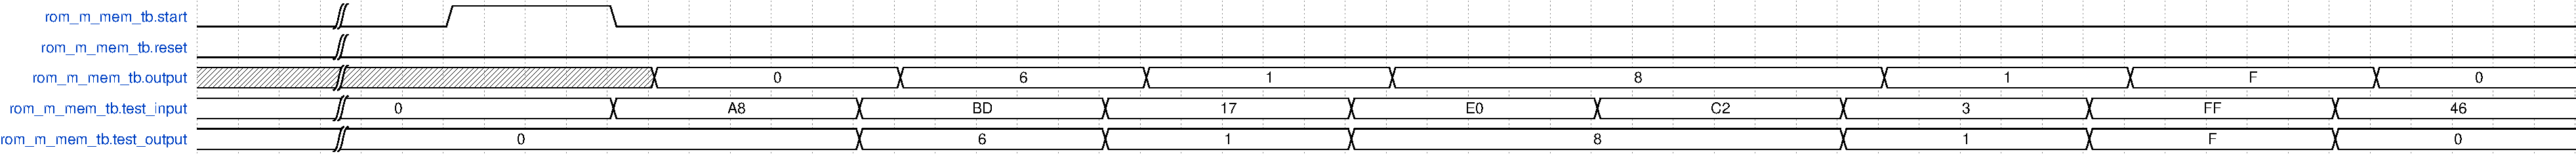
\includegraphics[width=\textwidth]{img/rom_m_mem_tb.pdf}
    \caption{Simulazione del sistema di lettura-elaborazione-scrittura}
    \label{fig:rom_m_mem_tb}
\end{figure}

\subsection{Esercizio 6.2}
Si implementa un sistema hardware che legga dati da una memoria ROM, li elabora tramite un'unità combinatoria (\texttt{M}) e visualizza il risultato attraverso i LED di una scheda FPGA:
\begin{itemize}
    \item \texttt{BTNC} (pulsante centrale): avvia il processo (segnale \texttt{start}).
    \item \texttt{BTNU} (pulsante in alto): resetta il sistema.
    \item \texttt{LED} (4 bit): mostra l'output trasformato della macchina combinatoria \texttt{M}.
\end{itemize}

\begin{code}
    \inputminted{vhdl}{vhdl/rom_m_mem_onboard.vhd}
    \caption{Implementazione del sistema di lettura-elaborazione-scrittura su board}
    \label{cod:rom_m_mem_onboard}
\end{code}

\paragraph{Funzionamento generale.}
Il sistema funziona nel seguente modo:

\begin{enumerate}
    \item All'accensione, il sistema è fermo.
    \item Premendo il pulsante centrale (\texttt{BTNC}), il sistema legge sequenzialmente i dati dalla ROM e li trasforma.
    \item L'output trasformato viene visualizzato sui LED.
    \item Ogni secondo, un nuovo valore appare sui LED (grazie al clock rallentato).
    \item Premendo \texttt{BTNU}, il sistema si resetta.
\end{enumerate}

\paragraph{Struttura del codice.}
L’architettura è \texttt{structural}, ovvero il sistema è composto da diversi moduli interconnessi:

\begin{enumerate}
    \item \texttt{rom\_m\_mem\_onboard} [Codice sorgente \ref{cod:rom_m_mem_onboard}]:
    \begin{itemize}
        \item Legge i dati da una ROM (con N locazioni, ciascuna di 8 bit).
        \begin{itemize}
            \item \texttt{BTNC}: pulsante che fornisce il segnale di \texttt{start}.
            \item \texttt{BTNU}: pulsante di reset.
        \end{itemize}
        \item Li elabora tramite M, che li converte in 4 bit.
        \item Scrive il risultato in MEM.
        \item Riceve un segnale di clock lento per permettere la visualizzazione sui LED.
        \begin{itemize}
            \item \texttt{CLK100MHZ}: clock di ingresso a 100 MHz.
            \item \texttt{LED}: 4 LED (bit 15--12 del vettore \texttt{std\_logic\_vector(15 downto 12)}) per visualizzare l’output.
        \end{itemize}
    \end{itemize}
    \item \texttt{clock\_divider} [Codice sorgente \ref{cod:clock_divider}]: riduce la frequenza del clock da 100 MHz a 1 Hz, permettendo di vedere il cambiamento dei LED senza che avvenga troppo velocemente.
    \begin{itemize}
        \item \texttt{clock\_divided}: segnale che trasporta il clock rallentato da 100 MHz a 1 Hz.
    \end{itemize}
\end{enumerate}

Per poter utilizzare la board è stato necessario effettuare alcune modifiche al file dei constraints \texttt{Nexys A7-100T-Master.xdc}. In particolare, abbiamo dovuto aggiungere i seguenti vincoli:
\begin{itemize}
    \item Abilitare il clock a 100 MHz.
    \item Abilitare i pulsanti \texttt{BTNC} per il segnale di \texttt{start}, \texttt{BTNU} per il reset.
    \item Abilitare i LED \texttt{LED15}--\texttt{LED12} per la visualizzazione dell’output.
\end{itemize}
